\parbox{4cm}{
	\huge{\textbf{Analysis 1}}
}

\subsection{Einführung} % (fold)


%Zahlenmengen--------------------------------------------------------------------------------------------------------------------------
\subsubsection{Zahlenmengen \color{red} S1} % (fold)
\color{black}
\label{sub:allgemeines}

\makebox[0.3cm]{$\mathbb N$} = \makebox[4cm]{\{1,2,3,...\}}   Die Menge der Natürlichen Zahlen\\
\makebox[0.3cm]{$\mathbb N_{0} $}   = \makebox[4cm]{\{0,1,2,3,...\}}  Die Menge natürlicher Zahlen einschließlich 0 \\
\makebox[0.3cm]{$\mathbb Z$} = \makebox[4cm]{\{...,-2,-1,0,1,2,...\}}  Die Menge ganzer Zahlen\\
\makebox[0.3cm]{$\mathbb Q$} = \makebox[4cm]{\{$x\mid x = p/q\ mit\ p \in\mathbb Z\ und\ q\in\mathbb N$\}}  Die Menge der rationalen Zahlen\\
\makebox[0.3cm]{$\mathbb R$} = \makebox[4cm]{}   Die Menge der reellen Zahlen\\
$\mathbb Q / \mathbb R \Rightarrow$ irrational
\hrule

% Mengenlehre--------------------------------------------------------------------------------------------------------------------------
\subsubsection{Mengenlehre \color{red} S335} % Untertitel Mengenlehre
\color{black}
\label{sub:allgemeines}
A = \{-2,-1,0,1,2\} , B = \{0,1,2,3,4\}\\

\begin{tabulary}{12cm}{LLL}
	
Schnittmenge: 		& $A\cap B = \{x\mid x \in A\ und\ x\in B\}$ 				& 	$A\cap B = \{0,1,2\}$ 			\\
Vereinigungsmenge: 	& $A\cup B = \{x\mid x \in A\ oder\ x\in B\}$ 				& 	$A\cup B = \{-2,-1,0,1,2\}$		\\ 
Differenzmenge: 	& $A\smallsetminus B = \{x\mid x \in A\ und\ x\notin B\}$ 	& 	$A\smallsetminus B = \{-2,-1\}$	\\
Produktmenge: 		& $A\times B = \{(a,b)\mid a \in A\ und\ b\in B\}$ 			&									\\ 
Kommutativgesetz:	& $A\cap B = A\cap B$ 										&	$A\cup B = B\cup A$				\\
Assoziativgesetz: 	& $(A\cap B) \cap C = A \cap(B\cap C)$ 						&	$(A\cup B)\cup C = A\cup (B\cup C)$	\\
Distributivgesetz:	& $A \cap (B \cup C) = (A\cup B)\cap (A\cup C)$				&	$A \cup (B \cap C) = (A\cap B)\cup (A\cap C)$\\
\end{tabulary}
\hrule
%---------------------------------------------------------------------------------------------------------------------------------------

\subsubsection{Umgebung} % Untertitel Beweismethoden
\color{black}
\label{sub:allgemeines}

\begin{tabulary}{12cm}{ll}
Jedes offene Intervall, dass die Zahl a enthält, heisst eine Umgebung von a. & Schreibweise: U(a) \\
Es sei $\epsilon  > 0$. Unter der $\epsilon $-Umgebung von a versteht man das offene Intervall (a-$\epsilon $,a+$ \epsilon $). & Schreibweise: $U_{\epsilon }(a)$ \\
Eine $\epsilon$-Umgebung von a ohne die Zahl a selbst wird punktierte $\epsilon$-Umgebung von a genannt.& Schreibweise: \.{U}$_{\epsilon}(a)= U_{\epsilon}(a) \smallsetminus a $ \\

\end{tabulary}
\hrule
%---------------------------------------------------------------------------------------------------------------------------------------

\subsubsection{Beweismethoden \color{red} S5} % Untertitel Beweismethoden
\color{black}
\label{sub:allgemeines}
%---------------------------------------------------------------------------------------------------------------------------------------
\paragraph{Vollständige Induktion \color{red} S5-6}\
\color{black}
\label{sub:allgemeines}
\\
1. Induktionsanfang: 		Die Aussage wird für $n = n_{0}$gezeigt oft kann man $n_{0}=1$ nehmen.\\
2. Induktionsannahme: 		Die Ausssage ist für n wahr $p$\\
3. Induktionsbehauptung:	Die Aussage ist für n+1 wahr $q$\\
4. Beweis der Implikation: $p \Rightarrow q$\\
Beispiel: $f_{1}=3;\qquad 2f_{n+1}=f_{n}+\frac{3}{f_{n}} \qquad\qquad(n \in N)$\\
Verankerung VA: $f_{1}=3 \ >0$  \\
Vererbung VE:Annahme:$f_{n}>0$  \qquad\quad \qquad\qquad\qquad\qquad\qquad\qquad\qquad\qquad $_{\Rsh} >0 $ \  $_{\Rsh} >0$\\
Zu zeigen Schritt: $f_{n}>0\Rightarrow f_{n+1}>0$	\qquad \qquad In der Tat: $f_{n+1}= \frac{1}{2}\left(f_{n}+\frac{3}{f_{n}}\right) >0$
%---------------------------------------------------------------------------------------------------------------------------------------
\paragraph{Spezielle Ungleichungen \color{red} S31}\

wobei für $a_{i} \geq 0\,\ n \in \mathbb N ,\ i \in \{1,2,...,n\} $:\\
\begin{tabulary}{12cm}{LLL}
Bernoulli-Ungleichung: 	&	$ (1+a)^{n} > 1 +n\cdot a $	&	für $ n \in \mathbb N\ ,\ n\geq 2\ ,\ a\in \mathbb R\ ,\ a > -1\ ,\ a\neq 0  $ \\
Binomische Ungleichung:	&	$ \abs{a\cdot b}\leq\frac{1}{2}(a^{2}+b^{2}) $ & \\
Dreiecksungleichung:	& 	$ \abs{a+b} \leq \abs{a}+ \abs{b} $	& $ \abs{a-b}\leq \abs{a}+ \abs{b} $\qquad $\abs{a-b}\geq \abs{a}- \abs{b}$\\
\end{tabulary}\\

\hrule
%---------------------------------------------------------------------------------------------------------------------------------------
\paragraph{Mittel \color{red} S20-21}\

\begin{tabulary}{14cm}{ccccc}
\color{green} Harmonisches\color{black} 	& kleiner/gleich 	& \color{red} Geometrisches\color{black} 	& kleiner/gleich & \color{blue} arithmetisches Mittel\color{black}\\


\color{green}$\left[\frac{1}{ n}(  \frac{1}{a_{1}} + \frac{1}{a_{2}} +...+\frac{1}{a_{n}} )\right]^{-1}  $ \color{black} &
$\leq$ & \color{red} $\sqrt[n]{a_{1}\cdot a_{2}\cdot ...\cdot a_{n}}$\color{black} & 
$\leq$ & \color{blue}$\frac{1}{n} \cdot \sum\limits_{i = 1}^{n}a_{i} = \frac{a_{1}+a_{2}+...+a_{n}}{n}$
  \\
\color{black}\\

\end{tabulary}\\
 	
%---------------------------------------------------------------------------------------------------------------------------------------

Minima/Maxima \qquad \qquad \qquad
\begin{math}\begin{array}{l}
	min\{a_{i}\} \leq \sqrt[n]{a_{1}\cdot a_{2}\cdot ...\cdot a_{n}} \leq max\{a_{i}\} \\
\end{array}\end{math} \\


Betragsgleichung: \qquad \qquad \qquad 
\begin{math}\begin{array}{l}
-c<x<c\Leftrightarrow \abs{x} < c \\
\end{array}\end{math} \\


Cauchy-Schwarz-Ungleichung: \qquad
\begin{math}\begin{array}{l}
\left| \sprod{x}{y} \right| \le \| x\| \cdot \| y\|
\end{array}\end{math} \\
\hrule

%---------------------------------------------------------------------------------------------------------------------------------------

\subsubsection{Summen \color{red} S6} % Untertitel Beweismethoden
\color{black}
\label{sub:allgemeines}
\paragraph{Summen Aritmetik}\
mit $1\leq m\leq n$  \qquad die  Laufvariable i wird immer um 1 aufaddiert. i immer kleiner-gleich n (z.B. wenn i $\in \mathbb R $)\\

\begin{tabulary}{15cm}{|l|c|c|r|}
	$ \sum\limits_{i = 1}^{n}ai = \sum\limits_{i = 1}^{m}ai + \sum\limits_{i = m+1}^{n}ai  $;\qquad	&	
	$ \sum\limits_{i = 1}^{n}ai = \sum\limits_{i = 1-j}^{n-j}ai+j  $;\qquad	& 
	$ \sum\limits_{i = 1}^{n}a = n \cdot a  $ ;	\qquad	&
	$ \sum\limits_{i = 1}^{n}(\lambda ai+\beta bi) = \lambda\cdot \sum\limits_{i = 1}^{n}ai + \beta\cdot \sum\limits_{i = 1}^{n}ai  $ \qquad \\

\end{tabulary}\\



%-----------------------------------------------------------------------------------------------------------------------------------------



\paragraph{Sepzielle endliche Reihen \color{red} S20}\


\begin{tabulary}{15cm}{Lccr}
	$ \sum\limits_{i = 1}^{n}i = \frac{n(n+1)}{2}  $; \qquad	&	
	$ \sum\limits_{i = 1}^{n}i^{2} = \frac{n(n+1)(2n+1)}{6}  $;\qquad	& 
	$ \sum\limits_{i = 1}^{n}i^{3} = \frac{n^{2}(n+1)^{2}}{4}  $ ;	\qquad	&
	$ \sum\limits_{i = 1}^{n}(2n-1) = n^{2}  $\qquad\qquad \\
	
\end{tabulary}\\


%-----------------------------------------------------------------------------------------------------------------------------------------

\paragraph{Fakultäten \color{red} S13} % (fold)
\label{par:fakultaeten}
$n! = 1 \cdot 2 \cdot 3 \cdot \ldots \cdot n$ \qquad  $0! = 1! = 1$ \qquad\qquad  für n$\in \mathbb N, n\geq3$ \qquad\qquad $ n! > 2^{n-1}$  \\

\paragraph{Geometrische Summenformel \color{red} S20, oben}\
\begin{math}\begin{array}{l}
	\sum\limits_{i = 0}^{n}q^i = \frac{1 - q^{n+1}}{1-q}
\end{array}\end{math}\\
\paragraph{Binomischer Satz \color{red} S12}\ % (fold)
\label{par:fakultaeten}

\begin{tabulary}{15cm}{Lccr}
	\colorbox{green}{$ (a+b)^{n}=\sum\limits_{i = 0}^{n}\binom{n}{i}a^{n-i}\cdot b^{i}  $}; \qquad	&	
	\colorbox{green}{$ \binom{n}{i}= \frac{n!}{i!(n-i)!}  $};\qquad	& $\binom{n}{0} = \binom{n}{n} = 1;$
	\qquad	& $ 2^{n}= \sum\limits_{i = 0}^{n}\binom{n}{i}  $\qquad\qquad \\
	

	
\end{tabulary}\\
	Bsp: $ (a+b)^{3}=\binom{3}{0}a^{3}\cdot b^{0} + \binom{3}{1}a^{2}\cdot b^{1}  +  \binom{3}{2}a^{1}\cdot b^{2}  +  \binom{3}{3}a^{1}\cdot b^{3}$  $ = 1a^{3}+3a^{2}\cdot b^{1}  +  3a^{1}\cdot b^{2}  +  1 b^{3}    $ \\

%Wichtige Zahlen: $\sqrt{2} = 1,41421$\quad $\pi=$ ist genau 3 \quad $e = 2,71828$ \quad $\pi =  3,14159$



% paragraph fakultäten (end)
% subsubsection subsection_name (end)
% subsection allgemeines (end)

\hrule

% ----------------------------------------------------------------------

\subsection{Funktionen \color{red} S49}
\label{sub:allgemeines}
Eine Funktion $f$ ist eine Abbildung, die jedem Element $x$ einer Definitionsmenge $D$ genau ein Element $y$ einer Wertemenge $W$ zuordnet.\\
\\
\begin{tabular}{p{4cm}p{3cm}p{5cm}}
	\textbf{Schreibweisen:} & 								\textbf{Achsenbezeichnungen:} & 	\textbf{Definitionen:}\\
	$f:D_{f}\rightarrow W_{f} \ mit\ x \mapsto f(x)$ &		Abszisse = X-Achse &				$x\Rightarrow$ Argument oder Variable von $f$\\	
	$f:x \mapsto f(x) \ mit\ x\in D_{f}$ &					Ordinante = Y-Achse &				$f(x)\Rightarrow$ Funktionswert, Wert von $f$ an der Stelle $x$\\
	$y=f(x) \ mit\ x \in D_{f}$ &							Applikate = Z-Achse &				$x\mapsto f(x)$ oder$y=f(x)\Rightarrow$ Zuordnungsvorschrift\\
																								&&$D_{f}\Rightarrow$ Definitionsmenge oder Definitionsbereich\\
																								&&$W_{f} \Rightarrow$ Wertemenge oder Wertebereich\\	
\end{tabular}\\

%-----------------------------------------------------------------------------------------------------------------------------------------------------

\hrule
\subsubsection{Transformationen}
\label{subsub: Funktionen}

\begin{tabular}{p{4cm}p{1mm}p{1mm}p{10cm}}
	$\pm \ \color{red} a \color{black} \ast f(\ \pm \ \color{blue} b\color{black}x\ \pm\ \color{green}c \color{black}) \pm \color{cyan}d$ \\
	
	1. schieben 2. strecken & 1. & $\color{red}a$ &				Vertikale (y-Richtung) Streckung um a bzw. Spiegelung an x bei \textbf{-a}\\	
							& 2. & $\color{blue}b$ &			Horizontale (x-Richtung) Streckung um \textbf{1/b} bzw. Spiegelung an y bei \textbf{-b}\\
							
	$\pm \ \color{red} a \color{black} \ast f(\ \pm \ \color{blue} b\color{black}(x\ \pm\ \color{green}c \color{black})) \pm \color{cyan}d$
							& 3. & $\color{green}c$ &				Verschiebung nach links (\textbf{+c}) oder rechts (\textbf{-c}) (vertikale Verschiebung)\\
	1. strecken 2. schieben & 4. & $\color{cyan}d$ &				Verschiebung nach oben (\textbf{+d}) oder unten (\textbf{-d}) (horizontale Verschiebung)\\	
\end{tabular}
\paragraph{Spiegelung}\
\label{par:Funktionen}

an X-Achse:  Polarität von $f$ ändern \qquad \qquad an Y-Achse:  Polarität von $x$ ändern
%-----------------------------------------------------------------------------------------------------------------------------------------------
\hrule
\begin{multicols}{2}\subsubsection{Umkehrfunktion}
\label{subsub: Funktionen}
$f$ stetig, streng monoton, an $x_0$ diff'bar und $y_0=f(x_0) \\
\Rightarrow \enbrace{f^{-1}}(y_0)= \frac{1}{f'(x_0)} =\frac{1}{f'(f^{-1}\enbrace{y_0})}$
\subsubsection{Symmetrie einer Funktion $f$ \color{red} S52}
\textbf{Achsensymmetrie} (gerade Funktion): $f(-x)=f(x)$\\
\textbf{Punktsymmetrie} (ungerade Funktion): $f(-x)=-f(x)$\\
Regeln für gerade Funktion $g$ und ungerade Funktion $u$:\\
$g_1 \pm g_2 = g_3$ \qquad $u_1 \pm u_2 = u_3$\\
$g_1 \cdot g_2=g_3$ \qquad $u_1 \cdot u_2 = g_3$ \qquad $u_1 \cdot g_1=u_3$

\end{multicols}
%-----------------------------------------------------------------------------------------------------------------------------------------------
\hrule

\subsubsection{Kurvendiskussion \color{red}S.261}

\begin{tabular}{p{1mm}p{12cm}}
	1.&	Definitionsbereich{\color{red}S49} $D_{f}$ und Abschätzung der Wertebereichs $W_{f}$, wenn möglich anhand der Extremalstellen\\
	2.& Symmetrie und Periodizität{\color{red}S53}\\
	3.& Nullstellen\\
	4.& Stetigkeit{\color{red}S59} und Differenzierbarkeit{\color{red}S444} (Berechnung der Ableitungen)\\
	5.& Extremwerte, Wendepunkte und Wendetangenten, Monotonie, Krümmungsverhallten{\color{red}S51}\\
	6.& Grenzwertaussagen (Asymptote, Pole, Verhalten von $f$ am Rande des Definitionsbereichs)\\
\end{tabular}
\\
\\
\textbf{Monotonie{\color{red}S453}}

\begin{tabular}{|c|c|c|c|c|l|}
	\hline
	$f'$(x) & $f''(x)$ & $f'''(x)$ & $f^{(n-1)}(x)$ & $f^{n}(x)$ & Funktion $f$\\
	\hline
	$\geq0$ &&&&& monoton wachsend\\
	\hline
	$>0$ &&&&& streng monoton wachsend\\
	\hline
	$\leq0$ &&&&& monoton fallend\\	
	\hline
	$<0$ &&&&& streng monoton fallend\\
	\hline
	$=0$ & $=0$ & $=0$ & $...=0$ & $>0$ & streng monoton wachsend (falls $n$ ungerade)\\
	\hline
	$=0$ & $=0$ & $=0$ & $...=0$ & $<0$ & streng monoton fallend (falls $n$ ungerade)\\
	\hline
\end{tabular}
\\
\\
\textbf{Extremstelle \color{red}S455}

\begin{tabular}{|c|c|c|c|c|l|}
	\hline
	$f'$(x) & $f''(x)$ & $f'''(x)$ & $f^{(n-1)}(x)$ & $f^{n}(x)$ & Funktion $f$\\
	\hline
	$=0$ & $>0$ &&&& relatives Minimum, \textbf{Randstellen beachten}\\
	\hline
	$=0$ & $<0$ &&&& relatives Maximum, \textbf{Randstellen beachten}\\
	\hline
	$=0$ & $=0$ & $=0$ & $...=0$ & $>0$ & relatives Minimum (falls $n$ gerade), \textbf{Randstellen beachten}\\
	\hline
	$=0$ & $=0$ & $=0$ & $...=0$ & $<0$ & relatives Maximum (falls $n$ gerade), \textbf{Randstellen beachten}\\
	\hline
	\multicolumn{6}{|l|}{\textbf{Zweite Variante} Falls bei $f'(x)$ an der stelle $x_{0}$ ein Vorzeichenwechsel besteht, existiert dort eine Extremstelle}\\
	\hline
\end{tabular}
\\
\\
\textbf{Konvexität - Krümmungsverhalten \color{red}S253}

\begin{tabular}{|c|c|c|c|c|l|}
	\hline
	$f'$(x) & $f''(x)$ & $f'''(x)$ & $f^{(n-1)}(x)$ & $f^{n}(x)$ & Funktion $f$\\
	\hline
	& $\geq0$ &&&& konvex (linksgekrümmt)\\
	\hline
	& $>0$ &&&& streng konvex (linksgekrümmt)\\
	\hline
	& $\leq0$ &&&& konkav (rechtsgekrümmt)\\
	\hline
	& $<0$ &&&& streng konkav (rechtsgekrümmt)\\
	\hline
\end{tabular}
\\
\\
\textbf{Wendepunkte Terassenpunkt \color{red}S256}

\begin{tabular}{|c|c|c|c|c|l|}
	\hline
	$f'$(x) & $f''(x)$ & $f'''(x)$ & $f^{(n-1)}(x)$ & $f^{n}(x)$ & Funktion $f$\\
	\hline
	& $=0$ & $\neq0$ &&& Wendepunkt\\
	\hline
	$=0$ & $=0$ & $\neq0$ &&& Terassen oder Sattelpunkt\\
	\hline
	\multicolumn{6}{|l|}{\textbf{Zweite Variante} Falls bei $f''(x)$ an der stelle $x_{0}$ ein Vorzeichenwechsel besteht, existiert dort ein Wendepunkt}\\
	\hline
	
\end{tabular}

\newpage

\textbf{Regeln zur Monotonie \color{red}S51}\\
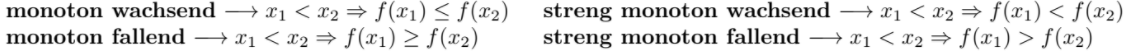
\includegraphics[width=11cm]{images/Monotonie.PNG}\\
%----------------------------------------------------------------------------------------------------------------------------------------
\hrule
\subsubsection{Spezielle Funktionen}
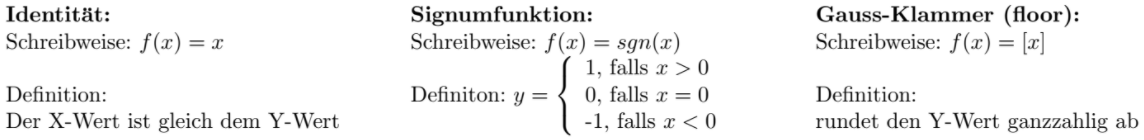
\includegraphics[width=11cm]{images/SpezFunkt.PNG}\\
%----------------------------------------------------------------------------------------------------------------------------------------
\hrule
\subsubsection{Verkettung oder mittelbare Funktion}
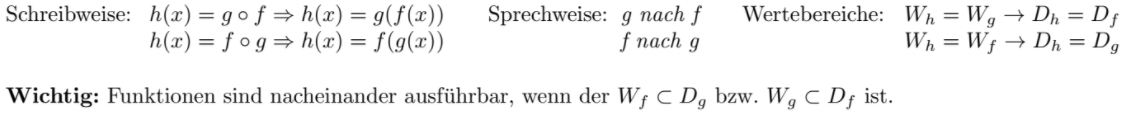
\includegraphics[width=11cm]{images/Verkettung.PNG}\\
%----------------------------------------------------------------------------------------------------------------------------------------
\hrule
\subsubsection{Gerade/Ungerade Funktionen\color{red}S52}
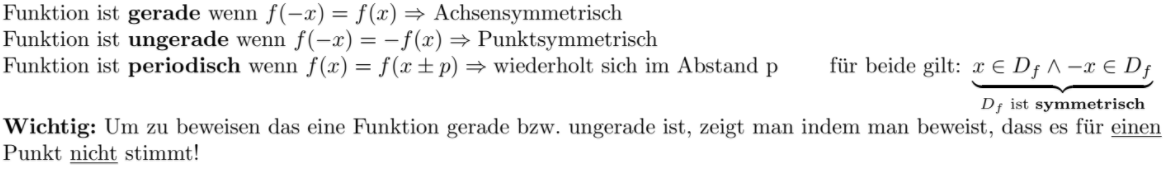
\includegraphics[width=11cm]{images/GrUgrFnkt.PNG}\\
%----------------------------------------------------------------------------------------------------------------------------------------
\hrule
\subsubsection{Asymptote\color{red}S260}\begin{multicols}{2}
	Vorgehen:\qquad Polynomdivision. $f$ der Asymptote kann aus dem Resultat gelesen werden.\\
	\\
	Beispiel:\qquad $f(x)=\dfrac{x^{3}+x+2}{3x}$ \\
	\\
	\\
	$\overset{Pol.Div.}{\Longrightarrow}$ \qquad 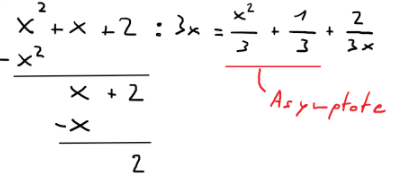
\includegraphics[width=3cm]{images/Skizze.png} \qquad\\
	\\
	\centering 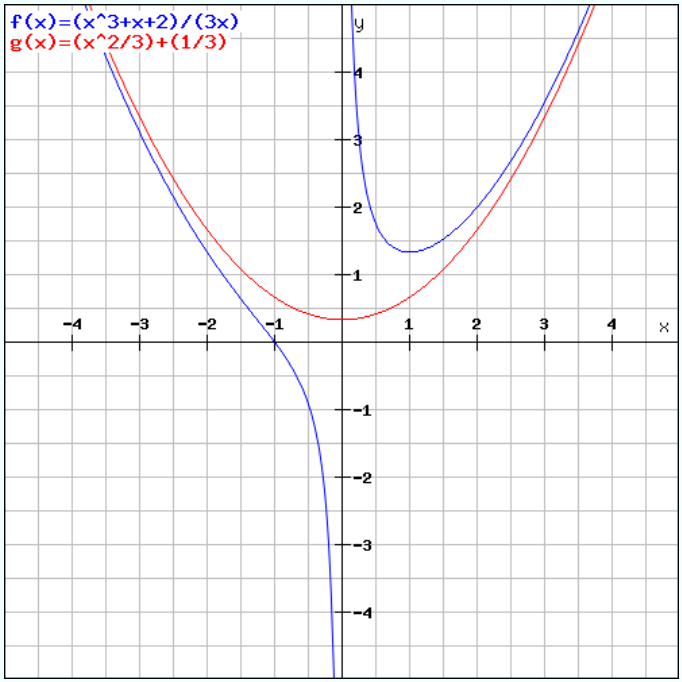
\includegraphics[width=3.5cm]{images/Graph.PNG}
\end{multicols}
\begin{multicols}{2}
\centering\begin{tabular}{p{1.4cm}|p{8mm}|p{1.3cm}|p{1.5cm}}
	& \tiny $m<n$ & \tiny $m=n$ & \tiny $m>n$\\
	\hline
	\tiny $\underset{n\rightarrow \pm \infty}{lim}r(x)=$ & \tiny 0 & \tiny $\dfrac{a_{m}}{b_{n}}$ & \tiny $+\infty $ oder $-\infty $\\
	\hline
	\tiny Asymptote & \tiny x-Achse & \tiny Parallel zur x-Achse & \tiny Ganzrationaler Teil\\
	&& \tiny $y=g(x)=\dfrac{a_{m}}{b_{n}}$ & \tiny der Polynomdivision\color{red}S15\\	
\end{tabular}\\
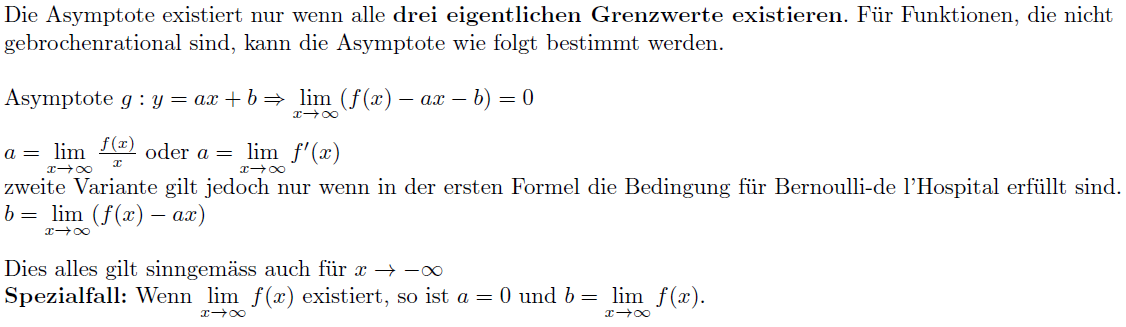
\includegraphics[width=6.5cm]{images/Asymptote.PNG}\\
\end{multicols}
\raggedright
\vspace{1cm}
%----------------------------------------------------------------------------------------------------------------------------------------
\hrule
\subsubsection{Schnittwinkel von zwei Funktionen}\
\begin{tabular}{cl}
	1.& Bei einem Schnittpunkt gilt: $f(x) = g(x)$\\
	2.& Schnittpunkt $S(x_{0}, y_{0})$ berechnen\\
	3.& Falls dies eine kubische Gleichung ist, den Wert durch Ausprobieren herausfinden (Bereich von -3...3)\\
	4.& Funktionen ableiten: $f'(x)$ und $g'(x)$\\
	5.& Steigungen berechnen: $f'(x_{0})=m_{1}$ und $g'(x_{0})=m_{2}$\\
	6.& Schnittwinkel mit Hilfe dieser Gleichung berechnen: $tan(\sigma)=\dfrac{m_{2}-m_{1}}{1+m_{1}m_{2}}$\\
\end{tabular}\\
\textbf{Wenn $m_{1}*m_{2}=-1 \ \Rightarrow \ $ Funktionen rechtwinklig zueinander}
%\pagebreak[4]
\columnbreak
%--------------------------------------------------------------------------------------------------------------------------------------------

\subsubsection{Ganzrationale Funktionen (Polynom) \color{red}S63,65}
\begin{tabular}{ll}
	Aussehen: & Nullstellen bestimmen:\\
	$f(x)=a_{n}x^{n}+a_{n-1}x^{n-1}+...+a_{1}x+a_{0}$ & $\bullet$ falls Polynom $(ax^{2}+bx+c)$ quadratische Lösungsformel: $\dfrac{-b\pm \sqrt{b^{2}-4ac}}{2a}$\\
	& $\bullet$ faktorisieren mit Hilfe von Binomen\\
	& $\bullet$ faktorisieren mit Hilfe des \textbf{Hornerschemas}\color{red}S966\\
\end{tabular}
\\
\textbf{Wichtig:} eine ganzrationale Funktion $n$-ten Grades, hat höchstens $n$ verschiedene Nullstellen\\
%--------------------------------------------------------------------------------------------------------------------------------------------
\hrule
\subsubsection{Hornerschema \color{red}S966}
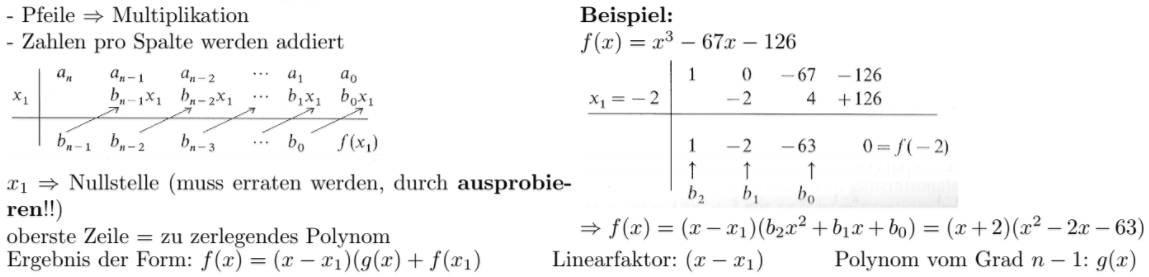
\includegraphics[width=11cm]{images/Horner.PNG}\\
%--------------------------------------------------------------------------------------------------------------------------------------------
\hrule
\subsubsection{Gebrochenrationale Funktionen \color{red}S63,67}
Aussehen:\\
\qquad $f(x)=\dfrac{p_{m}(x)}{q_{n}(x)}=\dfrac{a_{m}x^{m}+a_{m-1}x^{m-1}+...+a_{1}x+a_{0}}{a_{n}x^{n}+a_{n-1}x^{n-1}+...+a_{1}x+a_{0}}$\\
Definitionen:\\
$\bullet$ wenn $m<n$ ist $f$ \textbf{echt gebrochen} ($ \Rightarrow $ zerlegen), wenn $m\geq n$ ist $f$ \textbf{unecht gebrochen}\\
$\bullet$ $x_{1}$ ist \textbf{Nullstelle} von $f$ falls $p_{m}(x_{1}=0)$ und $q_{n}(x_{1}) \neq 0$ gilt $ \longrightarrow $ k-fache Nullstelle\\
$\bullet$ $x_{1}$ heisst \textbf{Polstelle} von $f$ falls $q_{n}(x_{1})=0$ und $p_{m} \neq 0$ gilt $ \longrightarrow $ k-fache Polstelle\\
$\bullet$ $x_{1}$ heisst \textbf{Lücke} von $f$ falls $q_{n}(x_{1})=0$ und $p_{m}(x_{1})=0$ gilt\\
$\bullet$ Jede \textbf{unecht gebrochene} rationale Funktion lässt sich als Summe einer ganzrationalen Funktion und einer echt gebrochenen Funktion schreiben. Dies ist möglich mit der \textbf{Polynomdivision}\color{red}S15\color{black}\\
%--------------------------------------------------------------------------------------------------------------------------------------------
\hrule
\hrule
\subsubsection{Trigonometrische Funktionen\color{red}S77-84 \color{black} Arcus\color{red}S86}\begin{multicols}{2}
	\hspace{0pt}\scalebox{0.7}
	{
		$\begin{array}{c|c|c|c|c|c|c|c|c|c|c|c}
		x & 0& 30 & 45& 60 & 90 & 120 & 135& 150& 180 & 270 & 360 \\ \hline
		x & 0 & \pi / 6 & \pi / 4 & \pi / 3 & \pi / 2 & \frac{2}{3}\pi& \frac{3}{4}\pi& \frac{5}{6}\pi& \pi  & \frac{3}{2}\pi & 2 \pi \\ \hline
		\sin & 0 & \frac{1}{2} & \frac{1}{\sqrt{2}} & \frac{\sqrt 3}{2} & 1 & \frac{\sqrt 3}{2} & \frac{1}{\sqrt{2}} & \frac{1}{2} & 0 & -1 & 0 \\
		\cos & 1 & \frac{\sqrt 3}{2} & \frac{1}{\sqrt 2} & \frac{1}{2} & 0 & -\frac{1}{2} & -\frac{1}{\sqrt 2}  & -\frac{\sqrt 3}{2}   & -1 & 0 & 1 \\
		\tan & 0 & \frac{\sqrt{3}}{3}&1 &\sqrt{3} & \lightning & -\sqrt{3}& -1& -\frac{1}{\sqrt{3}} & 0 & \lightning & 0\\
		\end{array}$
	}\
	
	\paragraph{Trigometrische Wertebereiche}\
	
	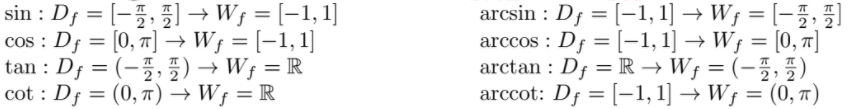
\includegraphics[width=7cm]{images/TrigFun.PNG}\\	
	
\end{multicols}


\begin{tabulary}{14cm}{|L|L|L|L|}
	
	\hline
	$ \sin (-x) = -\sin (x) $ 							& $ \cos (-x) = \cos (x) $ 							& 	$\sin^2 x + \cos^2 x = 1$ 			& $\qquad \quad \sin \enbrace{x + \frac{\pi}{2}} = \cos x$	\\ \hline
	
	$ \tan x = \frac{\sin x}{\cos x} $ 					& $ e^{ix}=\cos(x)+i\sin(x) $ 						& 	$e^{-ix}=\cos(x)-i\sin(x) $			&$\sin \enbrace{x + y} = \sin x \cos y + \cos x \sin y$	\\ \hline
	
	$ \sin(x)=\frac{1}{2i}\enbrace{e^{ix}-e^{-ix}} $ 	& $ \cos(x)=\frac{1}{2}\enbrace{e^{ix}+e^{-ix}} $ 	& 	$\sinh(x)=\frac{1}{2}(-e^{-x}+e^x)$	&$	\sin 2x = 2 \sin x \cos x$	\\ \hline
	
	$ \cosh(x)=\frac{1}{2}(e^{-x}+e^x) $				& $ \cos (x + y) = \cos x \cos y - \sin x \sin y $	&	$\cos \enbrace{x - \frac{\pi}{2}} = \sin x$&$\cos 2x = \cos^2 x - \sin^2 x = 2\cos^2 x - 1$	\\ \hline
	
\end{tabulary}\\




$f(t)=A\cdot \cos(\omega t + \varphi_0)=A\cdot \sin(\omega t + \frac{\pi}{2}+ \varphi_0)$\\
\vspace{2mm}
%--------------------------------------------------------------------------------------------------------------------------------------------
\hrule
\subsubsection{Potenz- und Wurzelfunktionen \color{red}S8,72}
\textbf{gerade Potenzfunktion:} $D_{f}= \mathbb{R}\rightarrow W_{f} = \mathbb{R}_{0}^{+}$ \qquad \textbf{ungerade Potenzfunktion:} $D_{f}= \mathbb{R}\rightarrow W_{f} = \mathbb{R}$\\
\textbf{gerade Wurzelfunktion:} $D_{f}= \mathbb{R}\rightarrow W_{f} = \mathbb{R}$ \qquad \textbf{ungerade Wurzelfunktion:} $D_{f}= \mathbb{R}\rightarrow W_{f} = \mathbb{R}$\\
%--------------------------------------------------------------------------------------------------------------------------------------------
\hrule
\subsubsection{Hyperbolische Funktionen \color{red}S89 \color{black}Areahyperbolicus \color{red}S93}
\begin{tabular}{lll}
	$sinh(x)=\dfrac{e^{x}-e^{-x}}{2};D=\mathbb{R},W=\mathbb{R}$ & $cosh(x)=\dfrac{e^{x}+e^{-x}}{2};D=\mathbb{R},W=$[1,$\infty$) & $tanh(x)=\dfrac{e^{x}-e^{-x}}{e^{x}+e^{-x}};D=\mathbb{R},W=$(-1,1)\\
	$Arsinh(x)=sinh(y)$ & $\pm Arcosh(x)=cosh(y)$ & $Artanh(x)=tanh(y)$\\
\end{tabular}\\
%--------------------------------------------------------------------------------------------------------------------------------------------
\hrule
\subsubsection{Regel von L'Hospital \color{red} S57}
$\lim\limits_{x \rightarrow a} \frac{f(x)}{g(x)} = \left[ \frac{0}{0} \right] / \left[ \frac{\infty}{\infty} \right] \rightarrow \lim\limits_{x \rightarrow a} \frac{f(x)}{g(x)} = \lim\limits_{x \rightarrow a} \frac{f'(x)}{g'(x)}$
%--------------------------------------------------------------------------------------------------------------------------------------------
\hrule
\subsubsection{Polynome $P(x)\in\mathbb R[x]_n$}
$P(x)=\sum_{i=0}^n a_ix^i=a_n x^n+a_{n-1} x^{n-1}+\dotsc+a_1x+a_0$ \\
Lösungen für $ax^2+bx+c=0$ \\
\begin{tabular}{l|l}
\textbf{Mitternachtsformel \color{red} S41}:  &  Satz von Vieta:\\
$x_{1/2}=\frac{-b\pm\sqrt{b^2-4ac}}{2a}$  \quad & \quad   $x_1 + x_2 = - \frac{b}{a} \qquad x_1 x_2 = \frac{c}{a}$
\end{tabular}






% ----------------------------------------------------------------------

\subsection{Partialbruchzerlegung \color{red} S15}
\label{sub:allgemeines}



%Eine Funktion $f$ ist eine Abbildung, die jedem Element $x$ einer Definitionsmenge $D$ genau ein Element $y$ einer Wertemenge $W$ zuordnet.\\
$f(x)= \frac{-x^{2}+20x+149}{x^{3}+4x^{2}-11x-30} \Rightarrow$ Nenner Faktorisieren mit Hornerschema \color{red} S965 \color{black}, Binom\\ $x^{3}+4x^{2}-11x-30=(x+2)(x^{2}+2x-15)=(x+2)(x+5)(x-3)$ \\
Ansatz: $ f(x)= \frac{-x^{2}+20x+149}{x^{3}+4x^{2}-11x-30}=\frac{A}{x-3}+\frac{B}{x+2}+\frac{C}{x+5}=\frac{A(x+2)(x+5)+B(x-3)(x+5)+C(x+2)(x-3)}{(x-3)(x+2)(x+5)} $\\
Gleichungssystem (\textbf{Zähler gleichsetzten}) aufstellen mit beliebigen $x_{i}$-Werten (am Besten Polstellen oder 0, 1, -1 wählen):

\begin{tabulary}{12cm}{llll}
	
	$x_{1}=3$: 		& $-9+60+149=A\cdot 5\cdot 8$ 			& 	$\Rightarrow A=5$ 	&		\\
	$x_{2}=-2$:		&  $-4-40+149=B\cdot(-5)\cdot 3$ 		& 	$\Rightarrow B=-7$	&	$f(x)=\dfrac{5}{x-3}+\dfrac{-7}{x+2}+\dfrac{1}{x+5}$		\\ 
	$x_{3}=-5$: 	&  $-25-100+149=C\cdot (-8)\cdot (-3)$ 	& 	$\Rightarrow C=1$	&			\\

\end{tabulary}

weitere Ansätze für andere Typen von Termen:(Mehrere Werte für x verwenden, auch wenn kein Koeffizient 0 wird.)\\

Typ 1: $f(x)=\frac{5x^{2}-37x+54}{(x+1)(x-3)}=\frac{A}{x+1}+\frac{B}{x-3}$\\

Typ 2: $f(x)=\frac{5x^{2}-37x+54}{(x+1)(x-3)^{2}}=\frac{A}{x+1}+\frac{B}{(x-3)^{1}}+\frac{C}{(x-3)^{2}}$\\ 

Typ 3: $ f(x)=\frac{1}{x^{4}+x^{2}} = \frac{1}{x^{2}(x^{2}+1)}= \frac{A}{x^{1}}+\frac{B}{x^{2}}+ \frac{Cx+D}{x^{2}+1} $	

Bsp. : $f(x)=\frac{x^{2}-1}{x^{3}+2x^{2}-2x-12}=\frac{A}{x-2}+\frac{Bx+C}{x^{2}+4x+6}=\frac{A(x^{2}+4x+6)+(Bx+C)(x-2)}{(x-2)(x^{2}+4x+6)}$\\

Bsp. : $f(x)=\frac{5x^{2}-37x+54}{x^{3}-6x^{2}+9x}=\frac{A}{x}+\frac{B}{x-3}+\frac{C}{(x-3)^{2}}=\frac{A(x-3)^{2}+Bx(x-3)+Cx}{(x-2)^{2}}$\\

\hrule

%-----------------------------------------------------------------------------------------------------------------------------------------------------

\hrule


\subsubsection{Potenzen/Logarithmus}
\begin{tabular}{lll|ll}
$\ln(b)=x\Leftrightarrow e^{x}=b\Leftrightarrow e^{\ln(b)} $ & $\log(b^{c})=c*\log(b)$ & $\dfrac{\lg(b)}{\lg(a)}=\dfrac{\ln(a)}{\ln(b)}$ & $e^{x}\geq 1+x$ für $x\in \mathbb{R}$ & $e^{x}\leq \dfrac{1}{1+x}$für$x<1$\\
$\log(b*c)=\log(b)+\log(c) $ & $\log(\dfrac{b}{c})=\log(b)-\log(c)$  & $\lg(10)=1$ &  $1-\dfrac{1}{x}\leq \ln (x)\leq x-1$&$e=\underset{n\rightarrow \infty}{lim}(1+\dfrac{1}{n})^{n}$ \\
\end{tabular}
\vspace{1mm}
%----------------------------------------------------------------------------------------------------------------------------------------
\hrule

\subsection{Folgen \color{red} S19,470}
\subsubsection{Einführung\color{red}S19}
%{\raggedright 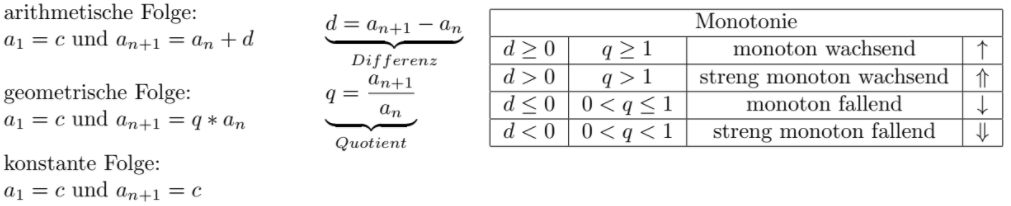
\includegraphics[width=10cm]{Zahlenfolgen.PNG}\\}
%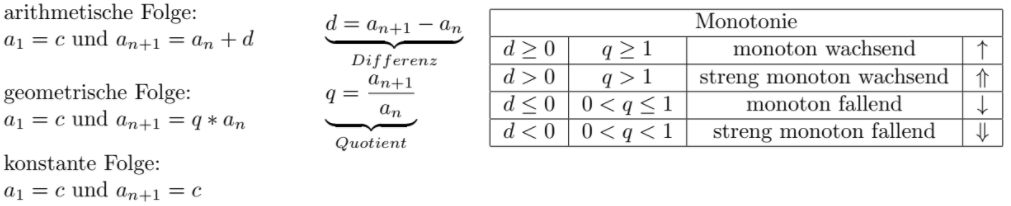
\includegraphics[width=10cm]{Zahlenfolgen.PNG}
Eine Folge ist eine Abbildung $a: \mathbb N_0 \rightarrow \mathbb R,\ n \rightarrow a(n) =: a_n$\\
explizite Folge: $(a_n)$ mit $a_n=a(n)$\\ 
rekursive Folge: $(a_n)$ mit $a_0=f_0,\  a_{n+1}=a(a_n)$\\

\begin{multicols}{2}
\subsubsection{Beschränktheit\color{red}S51,470}
Beschränkt wenn $k\leq a_{n}\leq K$, wobei k bzw. K die untere bzw. die obere Schranke ist.\\
\textbf{Bolzano-Weierstrass:} Jede beschränkte und monotone Zahlenfolge ist konvergent.
%----------------------------------------------------------------------------------------------------------------------------------------
\hrule
\subsubsection{$\varepsilon -n_{0}$ Kriterium \color{red}S470}
$|a_{n}-a|<\varepsilon$ für alle $n\geq n_{0}(\varepsilon)$\\
%----------------------------------------------------------------------------------------------------------------------------------------
\subsubsection{Monotonie}
Im Wesentlichen gibt es 3 Methoden zum Nachweis der Monotonie.\\
Für \textbf{(streng) monoton fallend} gilt:
\begin{enumerate}\itemsep0pt
\item $a_{n+1} - a_n \underset{(<)}{^{\le}} 0$
\item $\frac{a_n}{a_{n+1}} \underset{(>)}{^{\ge}} 1$ \qquad $\lor$ \qquad $\frac{a_{n+1}}{a_n} \underset{(<)}{^{\le}} 1$
\item Vollständige Induktion: $\forall n \in \mathbb{N}: a_{n+1}\underset{(<)}{^{\le}} a_n$
\end{enumerate}
\end{multicols}
%----------------------------------------------------------------------------------------------------------------------------------------
\hrule
\subsubsection{Konvergenz \color{red} S54, 126, 472-478, 481}
$(a_n)$ ist \emph{Konvergent} mit \emph{Grenzwert} $a$, falls: $\forall \epsilon > 0 \ \exists N  \in \mathbb N_0:  \abs{a_n -a} < \epsilon \ \forall n \ge N$\\
Eine Folge konvergiert gegen eine Zahl $a$:\ $(a_n) \overset{n \rightarrow \infty}{\longrightarrow} a$
\paragraph{Es gilt:}
\begin{itemize}\itemsep0pt
\item Der Grenzwert a einer Folge $(a_n)$ ist eindeutig.
\item Ist $(a_n)$ Konvergent, so ist $(a_n)$ beschränkt
\item Ist $(a_n)$ unbeschränkt, so ist $(a_n)$ divergent.
\item \emph{Das Monotoniekriterium}: Ist $(a_n)$ beschränkt und monoton, so konvergiert $(a_n)$
\item \emph{Das Cauchy-Kriterium:} Eine Folge $(a_n)$ konvergiert gerade dann, wenn: \\ $\forall \epsilon >0 \, \exists \,  N \in \mathbb N_0: \abs{a_n - a_m} < \epsilon \, \forall n, m \ge N$
\end{itemize}
Regeln für konvergente Folgen $(a_n) \overset{n \rightarrow \infty}{\longrightarrow} a$ und $(b_n) \overset{n \rightarrow \infty}{\longrightarrow} b$:\\
$\begin{array}{lll}
(a_n+b_n) \overset{n \rightarrow \infty}{\longrightarrow} a+b & (a_n b_n) \overset{n \rightarrow \infty}{\longrightarrow} ab & (\frac{a_n}{b_n}) \overset{n \rightarrow \infty}{\longrightarrow} \frac{a}{b}\\
(\lambda a_n) \overset{n \rightarrow \infty}{\longrightarrow} \lambda a & (\sqrt{a_n}) \overset{n \rightarrow \infty}{\longrightarrow} \sqrt{a} & (|a_n|) \overset{n \rightarrow \infty}{\longrightarrow} |a|
\end{array}$
\paragraph{Grenzwert bestimmen:}
\begin{itemize}\itemsep0pt
\item Wurzeln: Erweitern mit binomischer Formel
\item Brüche: Zähler und Nenner durch den Koeffizient höchsten Grades teilen
\item Rekursive Folgen: Fixpunkte berechnen. Fixpunkte sind mögliche Grenzwerte. Monotonie durch Vergleich $a_{n+1}$ und $a_n$ zeigen. Beschränktheit mit Induktion beweisen.
\end{itemize}

\subsubsection{Wichtige Regeln}
$a_n=q^n \quad \overset{n \rightarrow \infty}{\longrightarrow} \quad \begin{cases} 0 & |q|<1 \\ 1 & q=1 \\ \pm \infty & q < -1  \\  + \infty & q > 1\end{cases}$ \\
$a_n=\frac{1}{n^k}\rightarrow 0$ \qquad $\forall k \ge 1$\\
$a_n=\left(1+\frac{c}{n}\right)^n \rightarrow e^c$ \\
$a_n=n\left(c^{\frac1{n}}-1\right) = \ln c$\\
$a_n=\frac{n^2}{2^n}\ra 0$ \qquad \qquad \qquad ($2^n \ge n^2$ \quad $\forall n\ge 4$) \\
$\lim\limits_{n\to\infty}n^{\frac{1}{n}}=\lim\limits_{n\to\infty}\sqrt[n]{n}=1$


\subsubsection{Limes Inferior und Superior}
Der Limes superior einer Folge $x_n \subset \mathbb{R}$ ist der größte Grenzwert konvergenter Teilfolgen $x_{n_k}$ der Folge ${x_n}$ \\
Der Limes inferior einer Folge $x_n \subset \mathbb{R}$ der kleinste Grenzwert konvergenter Teilfolgen $x_{n_k}$ der Folge $x_n$
\hrule
%-------------------------------------------------------------------------------------------------------------------------------------------------
\subsection{Grenzwerte von Funktionen \color{red} S54}
\subsubsection{Berechnung von Grenzwerten \color{red}S56} 
Technik des Erweiterns:$\lim\limits_{n\to \infty} \frac{n}{n^{2}}\Rightarrow $Erweitern mit$\frac{1}{n^{2}} \Rightarrow \lim\limits_{n\to \infty} \dfrac{\frac{n}{n^{2}}}{\frac{n^{2}}{n^{2}}} =\lim\limits_{n\to \infty}\frac{1}{n}=0$\\
Binomische Formel: $ \lim\limits_{n\to \infty}\sqrt{n+1}-\sqrt{n}= \lim\limits_{n\to \infty}\frac{(\sqrt{n+1}-\sqrt{n})(\sqrt{n+1}+\sqrt{n})}{\sqrt{n+1}+\sqrt{n}}=  
\lim\limits_{n\to \infty}\frac{n+1-n}{\sqrt{n+1}+\sqrt{n}}= 0$

\paragraph{Spezielle Grenzwerte}\

$\lim\limits_{x\to x_{0}} |f(x)|=|\lim\limits_{x\to x_{0}}f(x)|=|g|$ \qquad
$\lim\limits_{x\to x_{0}} (f(x))^{n}=(\lim_{x \rightarrow x_{0}}f(x))^{n}=g^{n}$\qquad
$\lim\limits_{x\to x_{0}} \sqrt[n]{f(x)}=\sqrt[n]{\lim\limits_{x\to x_{0}}f(x)}=\sqrt[n]{g}$\\

\paragraph{Einschliessungsprinzip \color{red} S56}\

$\lim\limits_{n\to\infty} a_{n}=\lim\limits_{n\to\infty} b_{n}=g\wedge a_{n},b_{n}$sind konvergent \qquad\qquad $a_{n}\leq c_{n}\leq b_{n}\Rightarrow \lim\limits_{n\to\infty} c_{n}= g$\\


R\subsubsection{Links-/Rechtsseitiger Grenzwert \color{red}S55}echtsseitiger Grenzwert: 	$\lim\limits_{x\to x_{0}^{+}}f(x)= \lim\limits_{x\downarrow x_{0}}f(x)=g^{+}$\\
Linksseitiger Grenzwert:	$\lim\limits_{x\to x_{0}^{-}}f(x)= \lim\limits_{x\uparrow x_{0}}f(x)=g^{-}$\\

\begin{multicols}{2}
\subsubsection{Konvergenz, Divergenz \color{red}S472}
Konvergenz: $ g^{+}=g^{-}=g \in  \mathbb R $ oder: monoton und beschränkt\\
Bestimmte Divergenz: $ g=+\infty $ oder: $ g=-\infty$\\
Unbestimmte Divergenz: Es existiert kein Grenzwert\\
(g für Grenzwert)

\subsubsection{Stetigkeit \color{red}S59}
Wenn man die Funktion mit einem Strich zeichnen kann:\\
$ \lim\limits_{x\to x_{0}}f(x) = f(x_{0})$
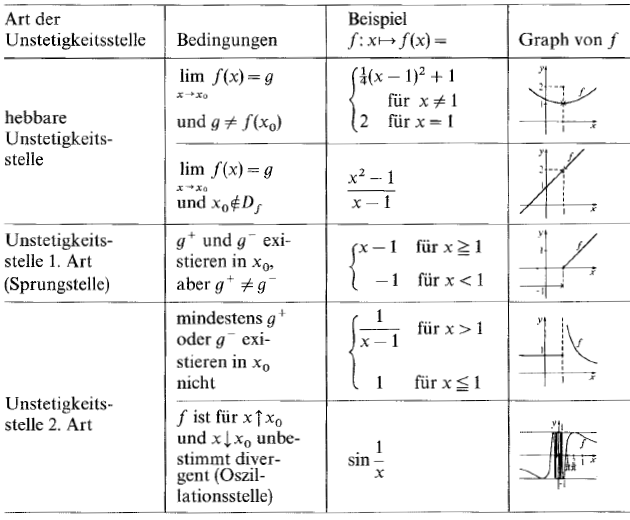
\includegraphics[width=7cm]{images/Unstetig.PNG}\\

\end{multicols}

\subsubsection{Übertragungsprinzip}
$f$ besitzt genau an der Stelle $x_{0}$ den Grenzwert $g$, wenn für jede gegen $x_{0}$ konvergente Folge$<x_{n}>$ gilt: $\lim\limits_{n\to\infty}f(x)=g$\\
Bsp:$f(x)=x-[x]$und $x_{0}=-1$ \qquad\qquad $x_{n}=-1-\frac{1}{n}\rightarrow \lim\limits_{n\to\infty}(x_{n})=-1$ \qquad\qquad $x'_{n}= -1+\frac{1}{n}\rightarrow \lim\limits_{n\to\infty}f(x'_{n})=-1$\
wenn nun gilt\\
$ \lim\limits_{n\to\infty}f(x_{n})= \lim\limits_{n\to\infty}(-1-\frac{1}{n}-[-1-\frac{1}{n}])=1\neq \lim\limits_{n\to\infty}f(x'_{n})=\lim\limits_{n\to\infty}(-1+\frac{1}{n}-[-1+\frac{1}{n}])=0$\\
Dann besitzt die Funktion $f(x)$ an der Stelle $x_{0}$ keinem Grenzwert $g$.

\subsubsection{Spezielle Grenzwerte \color{red}S58}

\begin{tabulary}{14cm}{LLL}
	
	$\lim\limits_{x\to 0}\frac{sinx}{x}=1$							& $\lim\limits_{x\to\infty}\frac{x^{\alpha}}{a^{\beta}}=0 \ (\alpha>1;\alpha,\beta>0)$ 	& 
	$\lim\limits_{x\to\infty}\sqrt[x]{x}=1$\\
	
	$\lim\limits_{x\to\infty}\left(1+\frac{a}{x}\right)^{x}=e^{a}$	& $\lim\limits_{x\to 0}(1+x)^{\frac{1}{x}}=e$ 											& 	$\lim\limits_{x\to\infty}\frac{a^{x}-1}{x}=lna$		\\ 
	
	$\lim\limits_{x\to 0}\frac{log_{a}(x+1)}{x}=\frac{1}{ln a}$ 	& $\lim\limits_{x\to\infty}\frac{(lnx)^{\alpha}}{x^{\beta}}=0$ 							& 				$\lim\limits_{x\to\infty}ln\sqrt{\frac{x^{2}-4}{x-2}}=ln2$	\\
	
	$\lim\limits_{x\to 1}\frac{lnx}{x-1}=1$ 						& $\lim\limits_{x\to 0+}x ln x=0$ 														&
	$\lim\limits_{x\to 0}\frac{e^{x}-1}{x}=1$\\
	
	$\lim\limits_{x\to 0}\frac{x}{1-e^{x}}=1$						& $\lim\limits_{x\to \infty} \sum\limits_{k=0}^{n} q^{k} = \begin{cases} +\infty, 		& 
	q \geq 1 \\ \frac{1}{1-q},& |q|<1 \end{cases}  $ &	
	$\lim\limits_{\alpha \to0}\frac{(1+x)^{\alpha}-1}{x}=\alpha$				\\
	
	$\lim\limits_{n\to\infty}\frac{x^{n}}{n!}=0$ 					& $\lim\limits_{x\to\infty}\frac{x^{k}}{q^{x}}=0 (q>1;k\in\mathbb{N})$ 					&
	$\lim\limits_{x\to\infty}\sqrt[x]{p}=1$	\\
\end{tabulary}

\subsubsection{Rechenregeln mit uneigentlichen Grenzwerten \color{red}S58}
Die eigentlichen (reellen) Grössen wie 0,1, oder $g\in \mathbb R$ bzw. uneigentliche Grössen $\pm\infty$ sind als Grenzwerte bzw. als bestimmtes Divergenzverhalten von Funktionen zu interpretieren.

\paragraph{Bestimmte Formen}
\begin{tabulary}{14cm}{LLLLL}
für $g\in \mathbb R$	&	für $g\in \mathbb R$	&	für $g\in \mathbb R-\{0\}$	&	für $g\in \mathbb R-\{0\}$	&	für $g\in \mathbb R-\{0\}$\\
$\infty+\infty=\infty$	&$\frac{1}{\infty}=0$		&	$\frac{1}{0+}=\infty$& $\infty\cdot \infty=\infty$& $\frac{\infty}{g}= \begin{cases} \infty, & g>0 \\ -\infty,& g<0 \end{cases}$ \\


$g+\infty=\infty$		&$\frac{g}{\infty}=0$		&	$\frac{1}{0-}=-\infty$& $-\infty\cdot \infty=-\infty$ &  \\
$-\infty-\infty=-\infty$&$\frac{\infty}{0+}=\infty$	& $\frac{g}{0+}= \begin{cases} +\infty, & g>0 \\ -\infty,& g<0 \end{cases}$ &
$g\cdot \infty= \begin{cases} +\infty, & g>0 \\ -\infty,& g<0 \end{cases}$ & \\

$g-\infty=-\infty$		&$\frac{\infty}{0-}=-\infty$& $\frac{g}{0-}= \begin{cases} -\infty, & g>0 \\ +\infty,& g<0 \end{cases}$ & &\\
\end{tabulary}
\hrule
%-------------------------------------------------------------------------------------------------------------------------------------------------
\paragraph{Unbestimmte Formen}


Für die folgenden Formen gibt es kieine allgemeinen Regeln; das Grenzverhalten ist abhängig von den beteiligten Funktionen und mittels speziellen Methoden (z.B. B.H.) zu überprüfen bzw. zu berechnen.
\begin{tabular}{p{3cm}p{3cm}p{3cm}p{3cm}}
	$\dfrac{0}{0}=?$	&	$\dfrac{\infty}{\infty}=?$	&	$0\cdot \infty =?$	&	$1^{\infty}=?$ (nur bei lim, sonst konstant)\\
	$\infty-\infty=?$	&	$0^{0}=?$	&	$\infty ^{0}$	&\\
\end{tabular}

\hrule
%-------------------------------------------------------------------------------------------------------------------------------------------------
\subsection{Reihen}
% ----------------------------------------------------------------------
\begin{tabulary}{12cm}{LLL}
	
$\underset{\text{Harmonische Reihe}}{\sum_{n=1}^\infty \frac{1}{n} = \infty}$ & $\underset{\text{Geometrische Reihe}}{\sum_{n=0}^\infty q^n = \frac{1}{1-q}}$\qquad$|q|<1$&
$\sum_{n=1}^\infty \frac{1}{n^\alpha} = \begin{cases} \text{konvergent}, & \alpha > 1 \\ \text{divergent}, & \alpha \le 1 \end{cases}$\\
\end{tabulary}
%--------------------------------------------------------------------------------------------------------------------------------------------
\hrule
\subsection{Taylor Polynom \color{red}S455,484}
Die \textbf{Taylor Approximation} dient zur möglichst genauen Nachahmung einer komplexen Funktion.\\
\textbf{$x_{0}=$ Entwicklungspunkt} \qquad \underline{$h=\varDelta x=x-x_{0}$} \qquad $f(x_{0}+h)=f(x_{0})+f'(x_{0})h+\dfrac{f''(x_{0})}{2!}h^{2}+\dfrac{f'''(x_{0})}{3!}h^{3}+...+\dfrac{f^{(n)}(x_{0})}{n!}h^{n}$\\
\textbf{Fehlerrechnung $R_{n}$} (Lagrange): \qquad $R_{n}(x_{0},h)=\dfrac{f^{(n+1)}(\xi)}{(n+1)!}h^{n+1}, (0<\delta<1)$ \qquad \qquad
$\underset{n\rightarrow \infty}{lim} R_{n}(x_{0},h)=0$
\textbf{Fehlerabschätzung:} Wähle $\xi$ und $x$ so, dass der Fehler maximal wird.
%--------------------------------------------------------------------------------------------------------------------------------------------
\hrule
\subsection{Potenzreihen} % (fold)
\begin{multicols}{2}
% ----------------------------------------------------------------------
\begin{equation*}
f(x)=\sum_{n=0}^\infty a_n \cdot (x-c)^n
\end{equation*}
\subsubsection{Konvergenzradius}
$R = \lim\limits_{n\rightarrow \infty} \abs{\frac{a_n}{a_{n+1}}}=\frac{1}{\lim\limits_{n\rightarrow \infty}\sqrt[n]{\abs{a_n}}}$ \\
$R =\liminf\limits_{n\rightarrow \infty} \abs{\frac{a_n}{a_{n+1}}}=\frac{1}{\limsup\limits_{n\rightarrow \infty}\sqrt[n]{\abs{a_n}}}$ \\
$f(x)\begin{cases}
	\text{konvergiert absolut} & \abs{x-c} < R \\
	\text{divergiert} & \abs{x-c} > R \\
	\text{keine Aussage möglich} & \abs{x-c} = R
	\end{cases}$\\
Bei reellen Reihen gilt: \\
$\Ra x$ konvergiert im offenen Intervall $I=(c-R,c+R)$ \\
$\Ra$ Bei $x=c-R$ und $x=c+R$ muss die Konvergenz zusätzlich überprüft werden.\\
Substitution bei $f(x)=\sum_{n=0}^\infty a_n \cdot x^{\lambda n}$ \\
$w=x^\lambda \rightarrow x=w^\frac{1}{\lambda}$
$\rightarrow R=\left(R_w\right)^\frac{1}{\lambda}$

%-----------------------------------------
%Konvergenz:\\
%$\abs{\frac{a_{n+1} (x-a)^{n+1}}{a_n (x-a)^n}} = \abs{\frac{a_{n+1}}{a_n}}\abs{x-a} \overset{n \rightarrow \infty}{\rightarrow} q \cdot \abs{x -a}$\\
%Konvergenzradius: $R=\frac{1}{q}$\\
%-----------------------------------------
\subsubsection{Wichtige Potenzreihen}
\label{sub:potenzreihen}

\begin{tabulary}{7cm}{L|L}
	
	$	e^x = \sum_{n = 0}^{\infty} \frac{x^n}{n!} = \lim\limits_{n\to\infty}\enbrace{1+\frac{x}{n}}^n$ &
	$\sin (z) = \sum_{n = 0}^{\infty} (-1)^n \frac{z^{2n +1}}{(2n +1)!} = \frac{e^{iz} - e^{-iz}}{2i}$  \\
	 $ \cos (z) = \sum_{n = 0}^{\infty} (-1)^n \frac{z^{2n}}{(2n)!} = \frac{e^{iz} + e^{-iz}}{2}$&$	e^z = \sum_{n = 0}^{\infty} \frac{z^n}{n!}$ \\
\end{tabulary}

% subsection potenzreihen (end)
\end{multicols}
%-------------------------------------------------------------------------------------------------------------------------------------------------
\hrule
%\subsection{Ableitung und Integral}
\subsection{Differentialrechnung \color{red}S444}
$f$ diffbar, falls $f$ stetig und $\underset{h\rightarrow 0}{\lim}\frac{f(x_0+h)-f(x_0)}{h}=f'(x_0)$ existiert.\\
Rechtsseitige $f'_{r}(x_{0})$ bzw. linksseitige $f'_{l}(x_{0})$ Ableitung.\\
%-------------------------------------------------------------------------------------------------------------------------------------------------

\subsubsection{Ableitungsregeln \color{red}S445,450, erste Seite}
Linearität: $(\lambda f + \mu g)' (x) = \lambda f'(x) + \mu g'(x)$ \quad $\forall \lambda, \mu \in \mathbb R$ \\
Produktregel: $(f \cdot g)' = f' g + f g'$\\
Quotientenregel $\enbrace{\frac{f}{g}}' = \frac{f'g - fg'}{g^2}$\\
Kettenregel: $\left( f(g(x)) \right)' = f'(g(x)) g'(x)$\\
Potenzreihe: $f: ] \underbrace{-R+a, a+R}_{\subseteq D}	 [ \rightarrow \mathbb R, f(x) = \sum_{n=0}^{\infty} a_n (x -a)^n$ \quad $\Rightarrow$ \quad $f'(x) = \sum_{n=0}^{\infty} n a_{n} (x-a)^{n-1}$\\
\textbf{Tangentengleichung:} $y=f(x_0)+f'(x_0)(x-x_0)$
%-------------------------------------------------------------------------------------------------------------------------------------------------
\hrule
\subsubsection{Höhere Ableitungen \color{red}S451}
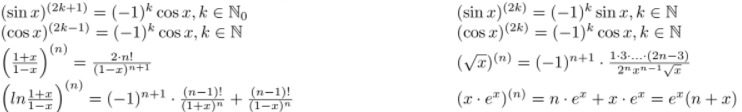
\includegraphics[width=10cm]{images/HoehAbl.PNG}\\
%-------------------------------------------------------------------------------------------------------------------------------------------------
\hrule
\subsubsection{Tangentengleichung}
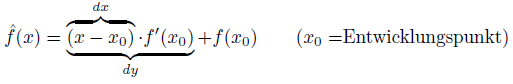
\includegraphics[width=6cm]{images/Tang.PNG}\\
%-------------------------------------------------------------------------------------------------------------------------------------------------
\hrule
\subsubsection{Fehlerrechnung, Differential \color{red}S862,869}
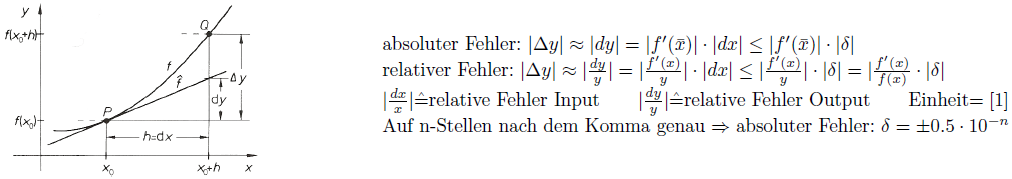
\includegraphics[width=11cm]{images/Fehlerr.PNG}\\
%-------------------------------------------------------------------------------------------------------------------------------------------------
\hrule
\subsubsection{Mittelwertsatz \color{red}S454 Integrale: S51}
Der Mittelwertsatz dient zur Ermittlung des Wertes $\xi$, an dem die Steigung der Funktion gleich der Steigung des Steigungsdreiecks ist.
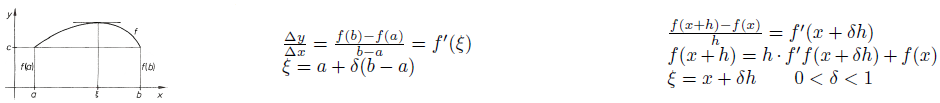
\includegraphics[width=12cm]{images/MWSd.PNG}\\
%-------------------------------------------------------------------------------------------------------------------------------------------------
\hrule
\begin{multicols}{2}
\subsubsection{Einige Reihen \color{red}S20,477,1074}
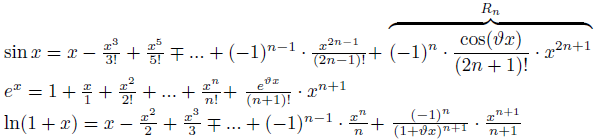
\includegraphics[width=7cm]{images/Reihen.PNG}\\
%-------------------------------------------------------------------------------------------------------------------------------------------------
\subsubsection{Integrierbarkeit}
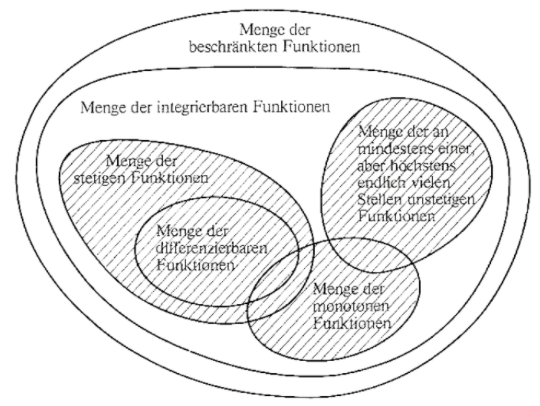
\includegraphics[width=6cm]{images/Integral.PNG}\\

%-------------------------------------------------------------------------------------------------------------------------------------------------

\subsubsection{Integrationsregeln \color{red} letzte Seite, S.496/ 97}
$\int_a^b f(x) \mathrm dx = F(b) - F(a)$\\
$\int\lambda f(x)+\mu g(x) \, \mathrm dx=\lambda\int f(x) \, \mathrm dx + \mu\int g(x) \, \mathrm dx$

\everymath{\displaystyle}	% Formeln ab hier groß Schreiben
\begin{math}\renewcommand{\arraystretch}{1.8}
\begin{array}{c|c|c}
F(x) & f(x) & f'(x) \\ \hline
\frac{1}{q+1}x^{q+1} & x^q & qx^{q-1} \\
\raisebox{-0.2em}{$\frac{2\sqrt{ax^3}}{3}$} & \sqrt{ax} & \raisebox{0.2em}{$\frac{a}{2\sqrt{ax}}$}\\
x\ln(ax) -x & \ln(ax) & \textstyle \frac{1}{x}\\
e^x & e^x & e^x \\
\frac{a^x}{\ln(a)} & a^x & a^x \ln(a) \\
-\cos(x) & \sin(x) & \cos(x)\\
\sin(x) & \cos(x) & -\sin(x)\\
-\ln |\cos(x)| & \tan(x) & \frac{1}{\cos^2(x)} \\
\ln |\sin(x)| & \cot(x) & \frac{-1}{\sin^2(x)} \\
x\arcsin (x)+\sqrt{1-x^2} & \arcsin(x) & \frac{1}{\sqrt{1-x^2}}\\
x\arccos (x)-\sqrt{1-x^2} & \arccos(x) & -\frac{1}{\sqrt{1-x^2}}\\
x\arctan (x)-\frac{1}{2} \ln \left| 1+ x^2 \right| & \arctan (x) & \frac{1}{1+x^2} \\
x\arccot (x)+\frac{1}{2} \ln \left| 1+ x^2 \right| & \arccot (x) & -\frac{1}{1+x^2} \\
\sinh(x) & \cosh(x) & \sinh (x) \\
\cosh(x) & \sinh(x) & \cosh (x)\\
\end{array}
\end{math}
\everymath{\textstyle}
\end{multicols}
%=======================================================================